\documentclass[aspectratio=43]{beamer}
\usepackage[latin1]{inputenc}
\usepackage{amsmath}
\usepackage{amsfonts}
\usepackage{amssymb}
\usepackage{makeidx}
\usepackage{graphicx}
\usepackage{array}

% Customization
\mode<presentation>{
\usetheme{CambridgeUS}
\usecolortheme{dolphin}
\setbeamertemplate{navigation symbols}{}
}

%\setbeamertemplate{footline}[frame number]

% Title and author
\title[QCD and Monte Carlo]{Quantum Coherent Phenomena}
\author{\textbf {Jes\'us Urtasun Elizari}}
%\institute{\textbf {University of Milan}}
\date{Milan, October 2020}

\begin{document}

% Front slide
\begin{frame}

	%\maketitle
	\vspace{1.0 cm}
	
	\center{\color{blue}Two-mode squeezed states in cavity optomechanics\\ via engineering of a single reservoir}
	
	\vspace{0.25 cm}
	\center{Quantum coherent phenomena course seminar - Milan, October 2020}

	\begin{figure}
		\minipage{1\textwidth}
		
\includegraphics[width = 3.0 cm]{plots/logo_unimi.png}
		\hfill
		
\includegraphics[width = 3.0 cm]{plots/logo_infn.png}
		\hfill
		
\includegraphics[width = 3.0 cm]{plots/logo_erc.png}
		\endminipage
	\end{figure}

	\vspace{1.0 cm}

\end{frame}

% Introduction
\begin{frame}

	\frametitle{Outline}
	
	\begin{enumerate}
		\item {\color{blue}Introduction}
		\item {\color{blue}System and Hamiltonian}
		\item {\color{blue}Reservoir engineering strategies}
		\item {\color{blue}Implementation}
		\item {\color{blue}Full system}
		\item {\color{blue}Experimental observability}
		\item {\color{blue}Two cavity modes, one mechanical oscillator}
	\end{enumerate}
	
\end{frame}

% Introduction
\begin{frame}

	\frametitle{Introduction}
	\framesubtitle{Entangled states}

	\begin{enumerate}
		\item Generation and detection of entangled states of macroscopic M.O
		\item Reservoir engineering $\longrightarrow$ Two-mode squeezed states. Bogoliuov modes
		\item Coherent feedback, steady state as EPR channel 
		\item Reservoir engineering studied in optomechanical systems. Krauter demonstrations (*)
	\end{enumerate}	
	
\end{frame}

% System and Hamiltonian I
\begin{frame}

	\frametitle{Introduction}
	\framesubtitle{System representation}
	
	\begin{columns}
		
		\column{0.5\textwidth}
		
		\begin{figure}
			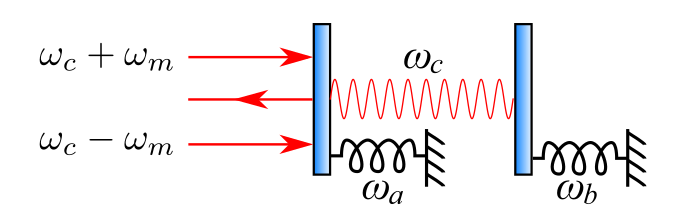
\includegraphics[width = 7 cm]{plots/plot_system.png}
		\end{figure}	

		\column{0.45\textwidth}

		\begin{itemize}
			\item Two mechanical oscillators, resonance frequencies $\omega_{a}, \omega_{b}$
			\item Dispersively coupled $g_{a}, g_{b}$ to a common cavity $\omega_{c}$
		\end{itemize}

	\end{columns}

\end{frame}

% System and Hamiltonian II
\begin{frame}
	
	\frametitle{Introduction}
	\framesubtitle{System representation}
	
	Hamiltonian of the system
	\begin{figure}
		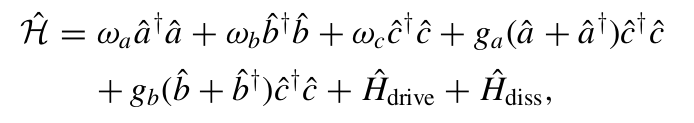
\includegraphics[width = 8 cm]{plots/hamiltonian_1.png}
	\end{figure}
	
	Under usual approximations, obtain the master formula 
	\begin{figure}
		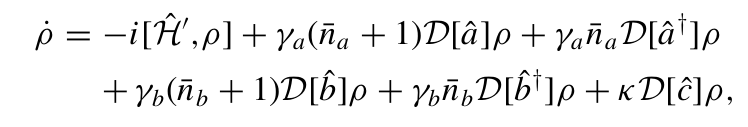
\includegraphics[width = 8 cm]{plots/master_eq_1.png}
	\end{figure}

	Being $\mathcal{D}$ dispersive superoperator, dampings and $\mathcal{H}'$
	
\end{frame}

% Reservoir engineering I
\begin{frame}
	
	\frametitle{Reservoir engineering strategies}
	\framesubtitle{Bogoliubov operators}
	
	2 mechanical oscillators. Modes $\hat{a}, \hat{b} \longrightarrow$ Bogoliuov operators 
	\begin{figure}
		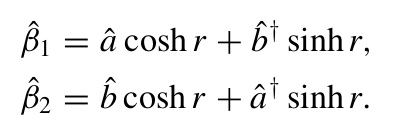
\includegraphics[width = 5 cm]{plots/bogoliubov_1.png}
	\end{figure}	

	Rotation with respect to some frame (*)
	\begin{figure}
		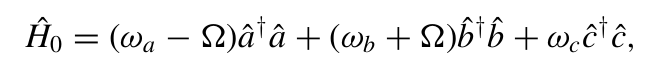
\includegraphics[width = 8 cm]{plots/hamiltonian_2.png}
	\end{figure}	

	Choice of $\Omega$ \\
	Collective mechanical quadratures (...)

\end{frame}

% Reservoir engineering II
\begin{frame}
	
	\frametitle{Reservoir engineering strategies}
	\framesubtitle{Ground state}
	
	2-mode squeezed state defined by $|r> = S_{2}(r) |00>$
	\begin{figure}
		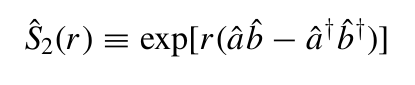
\includegraphics[width = 5 cm]{plots/2_squeezed_mode.png}
	\end{figure}	
	
	(...)
	
\end{frame}

% Reservoir engineering III
\begin{frame}
	
	\frametitle{Reservoir engineering strategies}
	\framesubtitle{Hamiltonian}
	
	Adding freq. difference between the mechanic oscillators, we break degeneracy of the Bogoliubov modes $\longrightarrow$ they couple to different frequency components of the reservoir 
	\begin{figure}
		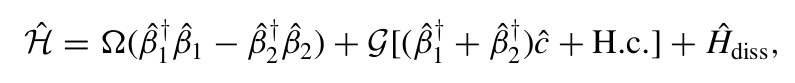
\includegraphics[width = 8.5 cm]{plots/hamiltonian_3.png}
	\end{figure}	
	
	where $\Omega$ is the effective frequency and $\mathcal{G}$ an effective coupling.
	\begin{columns} 
		
		\column{0.5\textwidth}
		
		In terms of the original operators
		\begin{figure}
			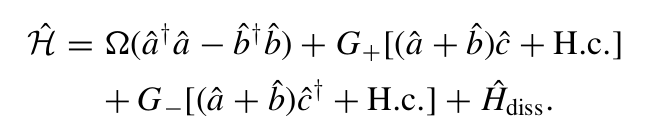
\includegraphics[width = 7.5 cm]{plots/hamiltonian_4.png}
		\end{figure}

		\column{0.5\textwidth}
		
		Optomechanical couplings\\
		related by
		\begin{figure}
			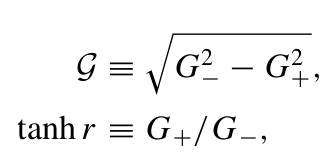
\includegraphics[width = 4 cm]{plots/optomechanic_couplings.png}
		\end{figure}

	\end{columns}

\end{frame}

% Reservoir engineering IV
\begin{frame}

	\frametitle{Reservoir engineering strategies}
	\framesubtitle{Goal}
	
	Engineer the driving Hamiltonian such that the squeezed-system results in $\hat{beta}_{i}$ cooled to their ground state.
	\begin{itemize}
		\item Experimental advantage
		\item Second method
		\item Third approach (*)
	\end{itemize}	

\end{frame}

% Implementation I
\begin{frame}

	\frametitle{Implementation}
	\framesubtitle{Different cases}
	
	Hamiltonian is already implemented in conventional optomechanical setups. Focus on regime $|G_{+}|<|G_{-}|$
	
	\begin{itemize}
		\item Two-tone driving ($g_{a} = g_{b}$)
		\item Four-tone driving ($g_{a} = g_{b}$)
		\item Case similar ($g_{a} \sim g_{b}$)
	\end{itemize}	
	
	(...)

\end{frame}


% Adiabatic limit I
\begin{frame}
	
	\frametitle{Adiabatic limit}
	\framesubtitle{Our system}
	
	Operator  $\hat{c} = -2i\mathcal{G}(\hat{\beta}_{1} + \hat{\beta}_{2})/k$\\
	Substitute into the dissipative terms of master equation $\longrightarrow$ adiabatically eliminated master equation
	\begin{figure}
		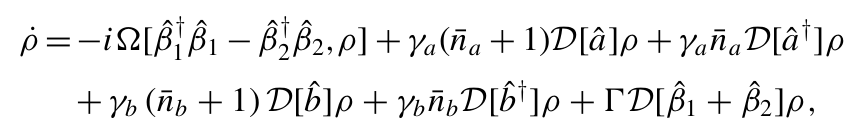
\includegraphics[width = 9 cm]{plots/master_eq_2.png}
	\end{figure}

	with optomechanical damping rate
	\begin{figure}
		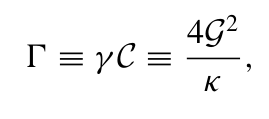
\includegraphics[width = 3 cm]{plots/optomechanic_dumping.png}
	\end{figure}
	
	Alternative view of the cooling of the Bogoliuov modes is possible (*)

\end{frame}

% Adiabatic limit II
\begin{frame}
	
	\frametitle{Adiabatic limit}
	\framesubtitle{Entanglement}
	
	Entanglement criterion using Duan inequality 
	\begin{figure}
		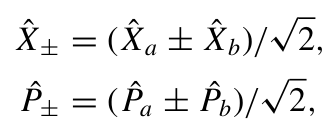
\includegraphics[width = 4 cm]{plots/entanglement_quad.png}
	\end{figure}	
	
	Where we introduced the quadrature modes as
	\begin{figure}
		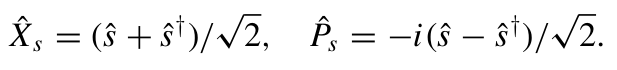
\includegraphics[width = 6.5 cm]{plots/entanglement_quad_2.png}
	\end{figure}

	Where we introduced the quadrature modes as
	\begin{figure}
		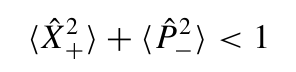
\includegraphics[width = 4 cm]{plots/entanglement_duan_criterion.png}
	\end{figure}

\end{frame}

% Adiabatic limit III
\begin{frame}
	
	\frametitle{Adiabatic limit}
	\framesubtitle{Entanglement}
	
	\begin{columns}
		
		\column{0.5\textwidth}
		
		\begin{figure}
			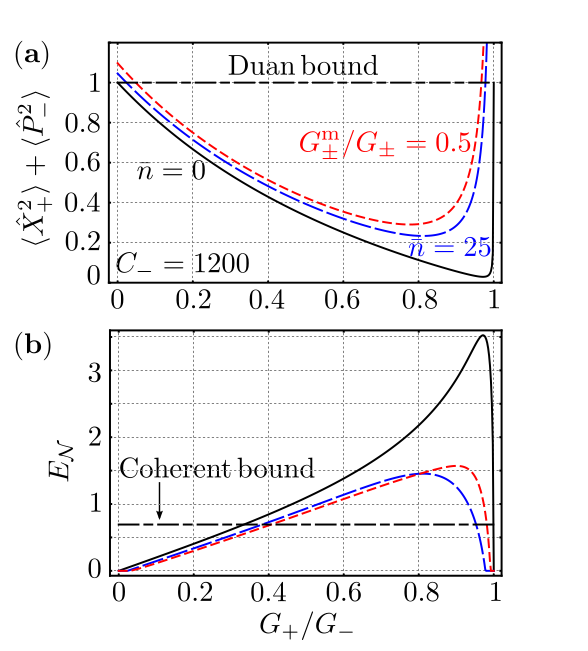
\includegraphics[width = 6 cm]{plots/plot_entanglement.png}
		\end{figure}	
	
		\column{0.65\textwidth}
		
		\begin{itemize}
			\item 1
			\item 2
			\item 3
		\end{itemize}
		
	\end{columns}

\end{frame}

% Adiabatic limit IV
\begin{frame}
	
	\frametitle{Adiabatic limit}
	\framesubtitle{Entanglement}
	
	\begin{columns}
		
		\column{0.5\textwidth}
		
		\begin{figure}
			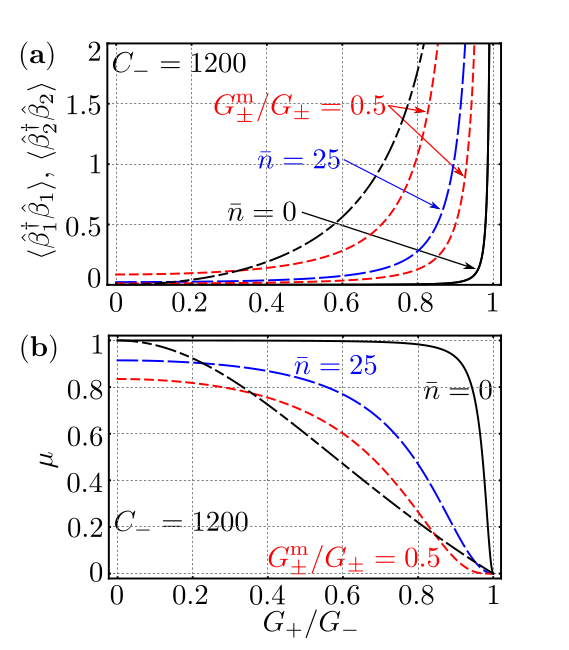
\includegraphics[width = 6 cm]{plots/plot_steady_state.png}
		\end{figure}	
		
		\column{0.65\textwidth}
		
		\begin{itemize}
			\item 1
			\item 2
			\item 3
		\end{itemize}
		
	\end{columns}

\end{frame}

% Conclusions
\begin{frame}

	\frametitle{Conclusions}
	
	\begin{enumerate}
		\item Configuring a three-mode optomechanical system such as the steady state includes highly pure and highly entangled two-mode squeezed state.
		\item Symmetry on the steady-state makes it attractive for implementation of  continuous-variable teleportation protocols
		\item Problem of unequal single-photon optomechanical couplings solved by using four-tone driving scheme
		\item Proposal implementable for existing technology
	\end{enumerate}
		
\end{frame}
\end{document}